 
\let\textcircled=\pgftextcircled
\chapter{Teoría Fractal} {\textit{Este capítulo describe un estudio sobre Teoría Fractal y su aplicación   al análisis de datos. }}
\label{cap:teoria_fractal}


\section{Consideraciones Iniciales}


\initial{E}l desarrollo de sistemas informáticos ha generado la necesidad del almacenamiento y procesamiento de tipos de datos complejos, tales como imágenes, vídeos, audio, datos biomédicos, hipertexto, etcétera. Estos datos son típicamente  voluminosos y con alta dimensionalidad. La mayoría de los enfoques utilizados en las técnicas mineras se basan en algoritmos con una complejidad computacional alta, tanto en el número de muestras como en el número de atributos (dimensiones) del conjunto de datos \cite{DMFractalsBook}.

 Un reto para la nueva generación de técnicas de minería de datos es descubrir hechos interesantes utilizando algoritmos escalables, es decir, algoritmos lineales o sublineales al menos tanto en el número de elementos como en el número de atributos del conjunto de datos. Por lo tanto, los investigadores de  base de  datos se esfuerzan en técnicas rápidas para la reducción de la dimensionalidad, el agrupamiento y la clasificación, así como las operaciones de indexación y recuperación asociados con otros procesos de minería de datos. Este capítulo aborda estos temas, específicamente el uso de la dimensionalidad intrínseca (o fractal) al análisis de los conjuntos de datos. Las técnicas basadas en fractales se adaptan bien a una muestra inicial de un conjuntos de datos, desde donde se pueden ejecutar analizadores más específicos y costosos. Además, las técnicas fractales tienden a seguir la percepción humana natural de las características del conjunto de datos mejor que la definición geométrica de los datos \cite{journals/jidm/TrainaTF10}. 
 
  
 En este capítulo presentamos los principales conceptos relacionados con la teoría fractal que son usados en algunos de los métodos propuestos en esta tesis. Presentamos un estudio de varias técnicas de análisis basadas en un conjunto de gráficos obtenidos a partir de conjuntos de datos mediante algoritmos de complejidad lineal basados en la teoría de fractales. Los gráficos proporcionan estimaciones sobre características significativas, tales como la dimensionalidad intrínseca   y la correlación  del conjunto de datos.  
 
 
 \section{Fractales}
Un fractal es definido como un objeto que presenta aproximadamente las mismas características independientemente de la escala donde es analizada, es un objeto que se parece a si mismo. Por otro lado, las partes del fractal son similares, exactas o estadísticamente  al  fractal completo. Esto es, a una escala mejor los detalles son similar a las características de una escala mayor \cite{Schroeder:1991,DMFractalsBook}.
 
Por ejemplo, el triangulo \textit{Sierpinkski} es un fractal geométrico, que ha sido construido en un proceso iterativo, teóricamente infinito.  En un triangulo equilátero ABC, donde primero se ha removido el triangulo central A', B', C',  de cada uno de los tres triángulos restantes cuyos lados longitud igual a la mitad del lado de ABC, retiramos de nuevo el triángulo central. La figura \ref{fig:ima1} muestra los pasos iniciales del proceso de construcción de un triángulo de $Sierpinski$. El triángulo restante tiene ``agujeros'' independientes de la escala y cada triángulo dentro de la primera es una ``miniatura'' de todo el triángulo.

\begin{figure}[h]
\centering
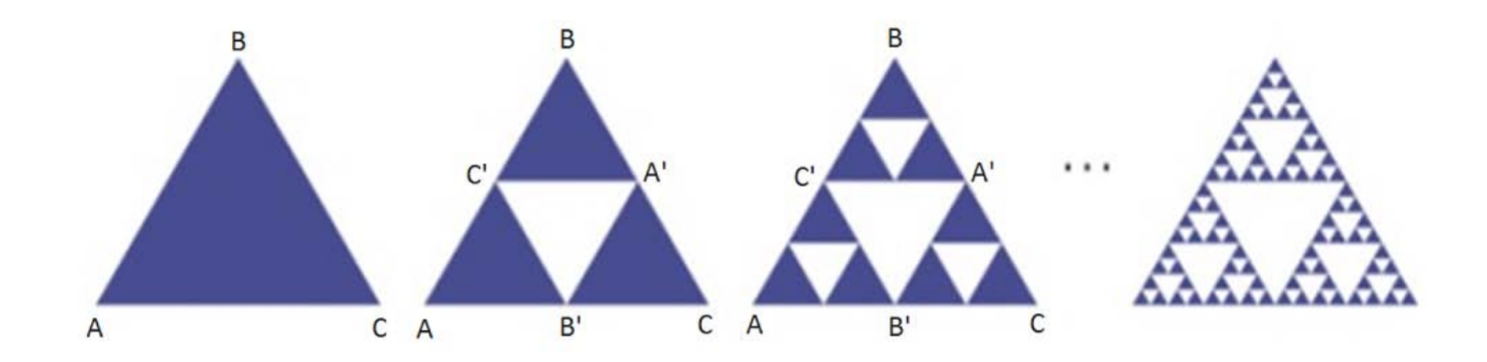
\includegraphics[scale=0.85]{chapter4/ima1.png}
\caption{Pasos del proceso de construcción del triangulo de $Sierpinsky$ \cite{DMFractalsBook}.}
\label{fig:ima1}
\end{figure}
Hay muchas otras estructuras matemáticas definidas como fractal, como las curvas de   $Koch$,  el conjunto de $Cantor$ y el conjunto de $Mandelbrot$ que son presentados en la figura \ref{fig:ima2}. Son también ejemplos de fractales en la naturaleza, por ejemplo: nubes, montañas, hortalizas, árboles, La costa de continentes, islas entre otros.
\begin{figure}[h]
\centering
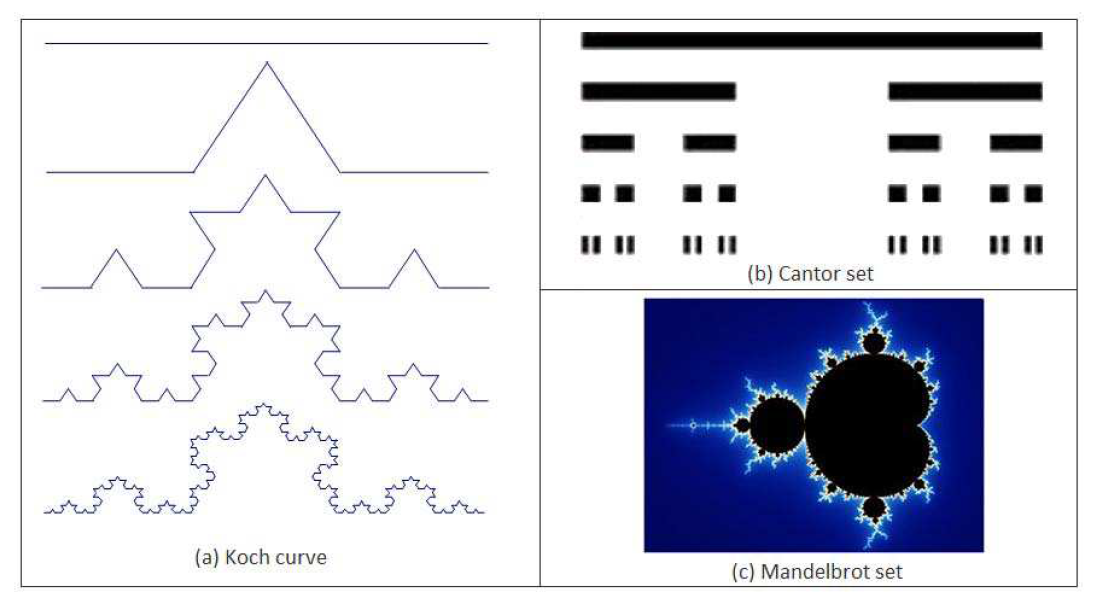
\includegraphics[scale=1.3]{chapter4/ima2.png}
\caption{Algunos ejemplos de fractales (a y b) fractales geométricos y (c) fractales algebraicos \cite{DMFractalsBook}.}
\label{fig:ima2}
\end{figure}


\section{Dimensión embebida y dimensión fractal}

Los conceptos de fractal se han aplicado a varias tareas en el análisis de datos y la minería de datos. Una de ellas es la estimación de la dimensión intrínseca (\mathfrak{D}) de un conjunto de datos, que es relacionado  con el concepto de dimensión embebida ($E$) \cite{conf/pods/FaloutsosK94}.

\begin{definition}{Dimensión embebida  $E$:} Dado un conjunto finito de datos $S$, la  
dimensión embebida $E \in N$ es el número de atributos que definen $S$. Es decir, $E$ es la dimensión de el espacio en el que se encaja el conjunto de datos.
\end{definition}}

\begin{definition}{Dimensión intrínseca $\mathfrak{D}$:} Dado un conjunto de datos finitos $S$, su dimensión intrínseca$\mathfrak{D} \in R^+$, es la dimensionalidad del objeto, independientemente de la
dimensión del espacio en el que está embebido.	
\end{definition}

La dimensión intrínseca ($\mathfrak{D}$) es una medida de la cantidad de información que el conjunto de datos representa. Por ejemplo, la dimensión intrínseca de un conjunto de puntos distribuidos a lo largo de una linea  es igual a uno; si el conjunto está embebido  en un espacio dimensional superior, la dimensionalidad intrínseca   continúa igual a uno tal como se ilustra en la Figura \ref{fig:ima3}.

\begin{figure}[h]
\centering
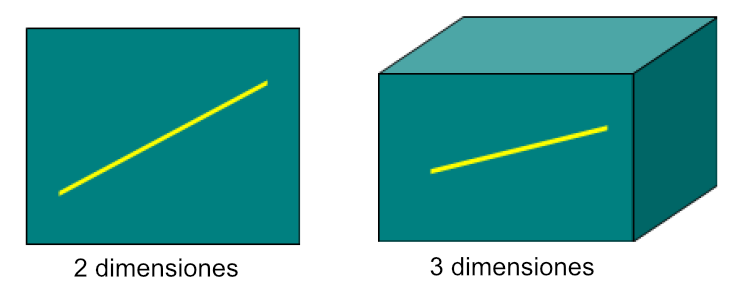
\includegraphics[scale=1.3]{chapter4/ima3.png}
\caption{Una linea embebida en dos o tres dimensiones donde $\mathfrak{D}=1$ \cite{DMFractalsBook}.}
\label{fig:ima3}
\end{figure}


\section{Dimensión fractal}

Faloutsos & Kamel (1994) \cite{conf/pods/FaloutsosK94} propusieron el uso de la dimensión intrínseca como una herramienta para medir el comportamiento no uniforme de conjuntos de datos reales. Además, los autores presentaron estudios empíricos para demostrar que los datos reales suelen tener un comportamiento de auto-similitud, que es  una   característica fundamental de los objetos fractales. Por lo tanto, la dimensión intrínseca $\mathfrak{D}$ de un conjunto de datos real puede calcularse usando la dimensión fractal \cite{journals/jidm/TrainaTWF10,DBLP:fractal2016}. La dimensión intrínseca basada en la dimensión fractal ha sido empleada como una herramienta para el análisis de agrupamiento \cite{Barbara2003},  reglas de asociación temporal \cite{Barbara2004}, selección de atributos \cite{journals/jidm/TrainaTF10}, series cronológicas \cite{Chakrabarti:2002:FLA:584792.584797} y la minería de datos espaciales \cite{Traina:2001:TST:502512.502538}.
 
Hay varias definiciones de la dimensión fractal, como veremos brevemente. En esta sección presentamos una visión general de algunos de ellos, introduciendo primero la dimensión fractal de fractales exactamente auto-similares.

\begin{definition}{Hausdorff Fractal Dimension $\mathfrak{D}_H$}
	
 Sea $M$ el número de réplicas y $s$ el factor de  escala
 por el que se reduce cada réplica, la dimensión fractal Hausdorff $\mathfrak{D}_H$ de un fractal auto-similar es   definido en un espacio $E$-dimensional como:
\begin{equation}
\mathfrak{D}_H = \lim_{s \to 0} (\frac{log M}{log (1/s)})
\label{eq:ec1}
\end{equation}

\end{definition}

Considere, por ejemplo, la dimensión fractal del triángulo de Sierpinsky, para la cual cada triángulo produce tres nuevos triángulos a media escala en cada paso, es decir, M = 3 y s = 1/2. Así,

$$	\mathfrak{D}_H = (\frac{log 3}{log 2}) = 1.58496  $$

La definición presentada en la Ecuación \ref{eq:ec1} se basa en la regla de construcción del fractal. Sin embargo, al medir la dimensión fractal de fractales estadísticamente autosimilares, que no presentan reglas de construcción explícitas, es necesario emplear un enfoque diferente, como el método de recuento de cajas (\textit{box-counting()}) \cite{journals/jidm/TrainaTF10}.
 
\section{Usando Gráficos  para estimar la Dimensión Fractal}

  De la teoría del fractal, la dimensión del fractal $\mathfrak{D}$ es particularmente útil para el análisis de datos, ya que puede aplicarse para estimar la dimensión intrínseca de conjuntos de datos reales que muestran un comportamiento fractal, es decir, exactamente o estadísticamente auto-similar \cite{Belussi:1995:ESS:645921.673166}. Se ha demostrado que, dado un conjunto de $N$ objetos en un conjunto de datos con una función de distancia $d(x,y)$, el número medio de $k$ vecinos dentro de una distancia dada $r$ es proporcional a $r$ elevado a $\mathfrak{D}$  \cite{Arantes_thefractal}.Así, la cuenta de pares $PC(r)$ de pares de elementos a distancia $r$ sigue la siguiente ley:
\begin{equation}\label{eq:fractal}
	   PC(r) = K_p \times r^{\mathfrak{D}}		
	\end{equation}
donde, $K_p$ es una constante proporcional  y $\mathfrak{D}$ es la dimensión fractal del conjunto de datos.     En consecuencia, un fractal es definido por la propiedad de auto-similitud, que es la característica principal que representa exactamente o estadísticamente la similitud entre las partes de todo el fractal.  

Si un conjunto de datos tiene un métrica para comparar cada par de sus elementos, se  puede dibujar un gráfico que lo represente, aunque el conjunto de datos no se encuentre en un dominio dimensional.  El trazado de este gráfico en escalas $log-log$, para la mayoría de los conjuntos de datos reales resulta en una línea casi recta para un rango significativo de distancias. Esta gráfica en la escala $log-log$   se llama la Diagrama de Distancia \cite{traina1999distance}. La pendiente de la recta en la gráfica de distancia es el exponente de la Ecuación \ref{eq:fractal}, por lo que se le llama Distancia Exponente. Es interesante notar que la dimensión intrínseca $\mathfrak{D}$ se aproxima mucho a la dimensión fractal  de un conjunto de datos.

    La Figura \ref{fig:mgcounty} muestra la gráfica de distancia de un conjunto de datos cuyos elementos son las coordenadas geográficas de las calles y carreteras del condado de Montgomery. Como se puede observar, las gráficas son lineales para el rango de tamaños más buscado en las consultas.  
\begin{figure}[h]
\centering
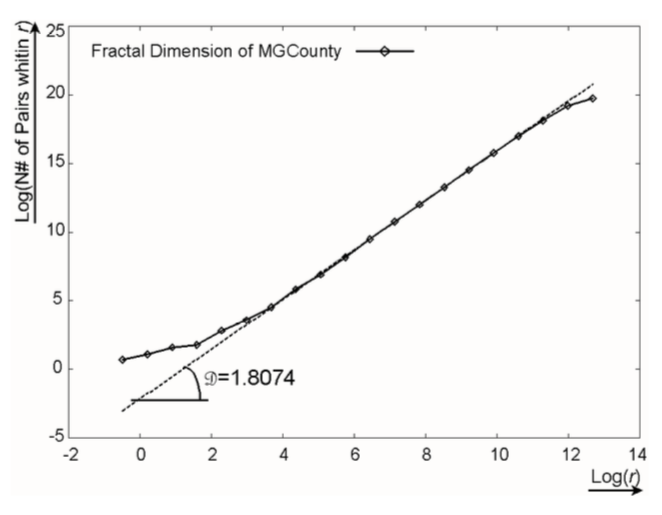
\includegraphics[scale=0.4]{chapter4/mgcounty.png}
\caption{Diagrama de Distancia para el conjunto de datos MgCounty mostrando una Dimensión Fractal $\mathfrak{D} \approx 1.81$ .}
\label{fig:mgcounty}
\end{figure}
	Utilizando gráficos como este, La Distancia Exponente $\mathfrak{D}$ de cualquier conjunto de datos puede calcularse como la pendiente de la recta que mejor se ajuste a la curva resultante en el Diagrama de Distancia. Por lo tanto, considerando la Figura \ref{fig:mgcounty}, la Ecuación \ref{eq:fractal} puede ser expresada como:
	
	\begin{equation}\label{eq:logpc_fractal}
	   log(PC(r)) = \mathfrak{D} \times log (r) + K_p 		
	\end{equation}
		La Distancia Exponente tiene muchas propiedades interesantes, derivadas de   la Dimensión Fractal. La propiedad principal es que la   dimensión fractal $\mathfrak{D}$ es invariante al tamaño del conjunto de datos, siempre que se utilice un número razonable de elementos de una muestra representativa  \cite{Faloutsos:2000:SJS:335191.335412}. Esto permite mantener el Distancia Exponente    para un conjunto de datos incluso después de que se haya actualizado el conjunto de datos con inserciones y eliminaciones.

 
\subsection*{Algoritmo de Calculo de la Dimensión Fractal}
 
 Una manera práctica de estimar $\mathfrak{D}$  a partir de un conjunto de datos espaciales está utilizando el método de  \textit{box-counting()} \cite{Faloutsos:2000:SJS:335191.335412}. Teóricamente, este método da una aproximación cercana a la dimensión fractal   \cite{traina1999distance}. Uno de los mejores algoritmos publicados para calcular la dimensión fractal  de un conjunto de datos es un algoritmo $O (N log (N))$, donde $N$ es el número de puntos en el conjunto de datos \cite{Belussi:1995:ESS:645921.673166}.   Sin embargo, existe un algoritmo aún más  rápido  de costo  $O (N)$  llamado \textit{box-counting()} \cite{journals/jidm/TrainaTF10}.
 
\section{Consideraciones Finales}

Las técnicas de minería de datos incluyen una amplia gama de herramientas de análisis, desde enfoques muy puntuales que intentan localizar características específicas de los datos, hasta herramientas muy amplias que sólo proporcionan una visión general de alto nivel de los datos. Sin embargo, la mayoría de los enfoques utilizados, independientemente de que sean específicos o amplios, se basan en técnicas basadas en algoritmos con una complejidad computacional  alta, tanto en el número de muestras como en el número de atributos (dimensiones) del conjunto de datos. Las técnicas presentadas en este capítulo, basadas en la teoría fractal, proporcionan algoritmos que pueden analizar datos en una complejidad computacional lineal tanto en el número de muestras como en el número de dimensiones. Estas técnicas están bien adaptadas a procesos amplios, por lo que pueden ser utilizadas como una muestra inicial en conjuntos de datos, desde los cuales se pueden ejecutar analizadores más específicos y costosos.

 

